\section{Method}
\label{sec:method}

\begin{figure}[!t]
    \centering
    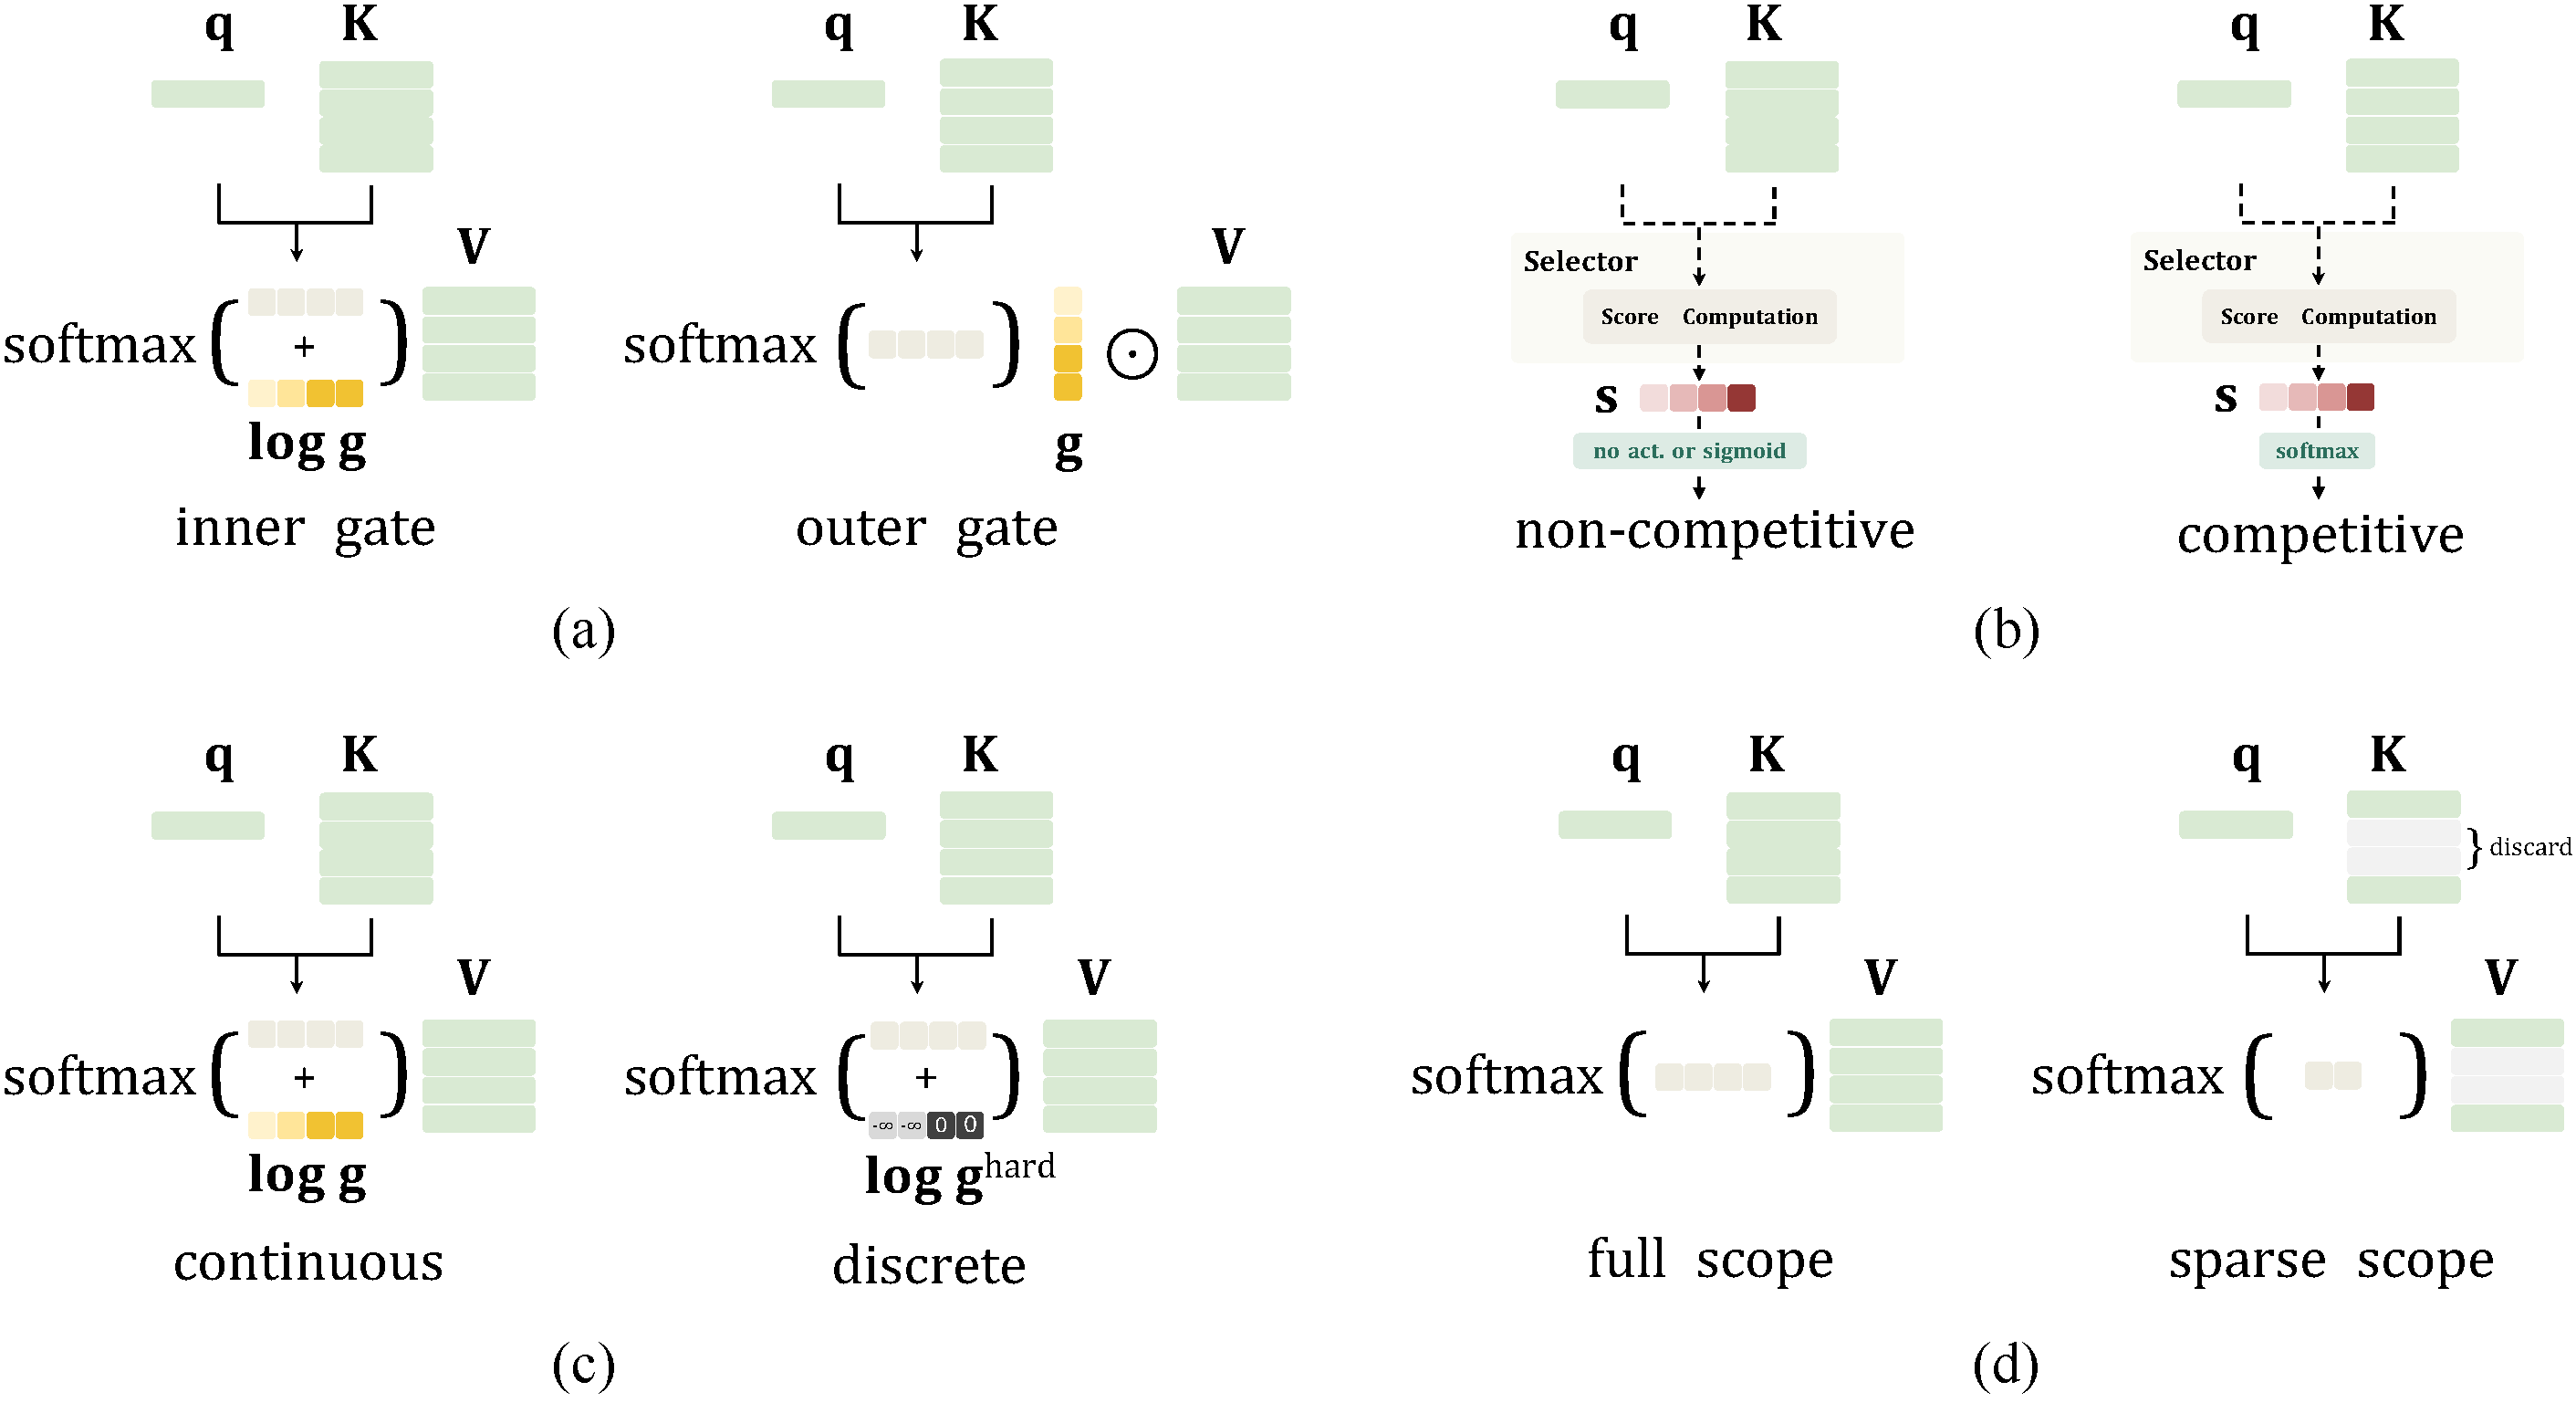
\includegraphics[width=0.93\linewidth]{sec/fig/all-abl2_cropped.pdf}
    \caption{Components of learnable context ranking.
    (a) Gate position, whether the gates are injected into the $\operatorname{softmax}$ or applied outside the $\operatorname{softmax}$.
    (b) Gate activation, whether historical-block scores are normalized jointly with $\operatorname{softmax}$, activated independently with $\operatorname{sigmoid}$, or injected as raw logits; the current block always has a unit gate.
    (c) Ranking preservation, whether continuous scores are preserved or collapsed into binary masks.
    (d) Training scope, whether training receives the gradient from all context blocks or only the selected blocks.}
    \label{fig:abla}
\end{figure}

We present \our, a \textbf{S}imple \textbf{A}ttention \textbf{S}parsification method that trains a lightweight selector to rank context blocks from the language modeling loss.
In this section, we first reformulate sparse block selection as context ranking.
We then analyze how to make such rankings learnable from the language modeling loss, focusing on gate position, gate activation, ranking preservation, and training scope.
Finally, we introduce a specialized training kernel for the practical implementation of \our.

\subsection{From Sparse Selection to Context Ranking}
\label{subse:context_rank}

The starting point is that Top-$K$ selection is determined by the ordering of selector scores over context blocks.
Before producing a discrete selected set, the selector first defines a ranking of candidate blocks.
A good selector should assign higher ranks to blocks that are more useful for prediction.
We therefore view attention sparsification as \emph{context ranking}: during training, the selector learns a continuous ordering over blocks, and this ordering provides the basis for sparse block selection.


\paragraph{Differentiable ranking.}
To make block ranking learnable, the selector scores must affect the attention computation during training.
Following the block partition in Section~\ref{sec:preliminary}, we single out the always-retained current block as $B_0$ and treat the remaining $C$ context blocks $\mathcal{H}=\{B_1,\ldots,B_C\}$ as the candidate historical blocks that the selector ranks.
The selector produces scores $\mathbf{s}\in\mathbb{R}^{C}$ only for $\mathcal{H}$, which we convert into positive gates
\begin{equation}
    \mathbf{g} = \phi(\mathbf{s})\in\mathbb{R}_{+}^{C},
    \qquad g_0=1,
    \label{eq:general_gate}
\end{equation}
where $\phi(\cdot)$ is a differentiable activation function and $g_0=1$ leaves the current block unbiased.
This transformation allows historical-block scores to modulate attention rather than determine a discrete Top-$K$ set.


For each historical block $B_m\in\mathcal{H}$, the gate $g_m$ is broadcast to all tokens in that block, while tokens in $B_0$ retain the unit gate.
By making the attention computation depend on these broadcast gates, gradients from the language modeling loss can flow back to $\mathbf{g}$ and then to the selector.
The key design question is how to \textit{integrate gates into the attention computation so that gradients provide a reliable signal for block ranking}.


\paragraph{Components of learnable ranking.}
Merely allowing language modeling gradients to reach the selector does not guarantee effective block ranking: different gated formulations shape the resulting ranking signals differently.
As illustrated in \Cref{fig:abla}, we investigate four design elements: gate position, gate activation, ranking information preservation, and training scope.

{\setlength{\leftmargini}{2em}
\begin{itemize}
 \item  \textit{Gate position}: whether the gates are applied into the $\operatorname{softmax}$, i.e., $\mathbf{o}_{\text{inner}}=\operatorname{softmax}(\mathbf{q}\mathbf{K}^{\top}+\log\mathbf{g})\mathbf{V}$, or applied outside the $\operatorname{softmax}$, i.e., $\mathbf{o}_{\text{outer}}=\operatorname{softmax}(\mathbf{q}\mathbf{K}^{\top})(\mathbf{g}\odot\mathbf{V})$. For the inner placement, $\log(\cdot)$ ensures that the gates act as multiplicative weights on the attention probabilities after the softmax.

 \item \textit{Gate activation}: how block scores are transformed before being injected into attention. We compare normalized gates $\mathbf{g}=\operatorname{softmax}(\mathbf{s})$, independent gates $\mathbf{g}_{\sigma}=\operatorname{sigmoid}(\mathbf{s})$, and unnormalized logit injection, which adds $\mathbf{s}$ directly to attention logits. In all variants, current block remains unbiased with $g_0=1$.

 \item \textit{Ranking preservation}: whether training uses a soft gate $\mathbf{g}=\phi(\mathbf{s})$, or a hard Top-$K$ gate using STE, i.e., $\hat{\mathbf{g}}=\operatorname{stopgrad}(\mathbf{g}^{hard}-\mathbf{g})+\mathbf{g}$ with $g^{hard}_m=\mathbb{I}[m\in\text{Top-}K(\mathbf{s},K)]$.

  \item \textit{Training scope}: whether training uses the full scope in Equation~\ref{eqn:fula}, the sparse scope in Equation~\ref{eqn:spa}, or a stochastic approximation to full scope by adding noise to the scores before activation.

\end{itemize}
}


\definecolor{avg}{HTML}{D05E46}
\begin{table}[!t]
\centering
\caption{
Ablation of four gating design choices on GPQA-Diamond using Qwen3-4B with a 2048-token budget. We report avg@16 accuracy (\%),
with \textcolor{avg}{average generation length}; standard deviations (2.0--2.8) are omitted. $\mathbf{g}_{\sigma}$ denotes sigmoid-activated gates, and full$^{*}$ simulates full-scope training by adding noise before Top-$K$. Formulations show only historical-context terms; the current block always uses a unit gate.
}
\label{tab:ablation_main}

\resizebox{\textwidth}{!}{
\newcommand{\res}[2]{#1~\textcolor{avg}{\scriptsize #2}}

\begin{tabular}{l cccc | cccc}
\toprule
\textbf{Setting} &
\textbf{Gate Pos.} &
\textbf{Gate Act.} &
\textbf{Rank Pres.} &
\textbf{Train Sco.} &
\textbf{10 step} &
\textbf{100 step} &
\textbf{1000 step} &
\textbf{1 epoch}
\\
\midrule

\multicolumn{9}{c}{\textit{Baseline}}\\
\midrule

(1) $\operatorname{softmax}(\mathbf q\mathbf K^\top)\mathbf V$ & -- & -- & -- & -- &
-- & -- & -- &
\res{56.1}{8547}\\

\midrule
\multicolumn{9}{c}{\textit{I. Gate Position (inner $\operatorname{softmax}$ vs. outer $\operatorname{softmax}$)}}\\
\midrule

(2) $\operatorname{softmax}(\mathbf q\mathbf K^\top+\log\mathbf g)\mathbf V$
& inner
& $\operatorname{softmax}$
& \checkmark
& full
& \res{30.8}{25277}
& \res{\textbf{52.2}}{8696\phantom{1}}
& \res{\textbf{53.7}}{6977\phantom{1}}
& \res{{54.4}}{7109\phantom{1}}
\\

(3) $\operatorname{softmax}(\mathbf q\mathbf K^\top)(\mathbf g\odot\mathbf V)$
& outer
& $\operatorname{softmax}$
& \checkmark
& full
& \res{28.3}{25594}
& \res{38.9}{16969}
& \res{43.2}{12801}
& \res{41.6}{13807}
\\

\midrule
\multicolumn{9}{c}{\textit{II. Gate Activation ($\operatorname{softmax}$, $\operatorname{sigmoid}$, or none)}}\\
\midrule

(4) $\operatorname{softmax}(\mathbf q\mathbf K^\top+\log\mathbf g)\mathbf V$
& inner
& $\operatorname{softmax}$
& \checkmark
& full
& \res{30.8}{25277}
& \res{\textbf{52.2}}{8696\phantom{1}}
& \res{\textbf{53.7}}{6977\phantom{1}}
& \res{{54.4}}{7109\phantom{1}}
\\

(5) $\operatorname{softmax}(\mathbf q\mathbf K^\top+\log\mathbf g_{\sigma})\mathbf V$
& inner
& $\operatorname{sigmoid}$
& \checkmark
& full
& \res{19.6}{27717}
& \res{20.4}{27997}
& \res{17.6}{27989}
& \res{17.0}{28444}
\\

(6) $\operatorname{softmax}(\mathbf q\mathbf K^\top+\mathbf s)\mathbf V$
& inner
& --
& \checkmark
& full
& \res{23.4}{27540}
& \res{19.9}{27418}
& \res{18.9}{26703}
& \res{18.8}{26401}
\\


\midrule
\multicolumn{9}{c}{\textit{III. Ranking Preservation (continuous vs. discrete)}}\\
\midrule

(7) $\operatorname{softmax}(\mathbf q\mathbf K^\top+\log\mathbf g)\mathbf V$
& inner
& $\operatorname{softmax}$
& \checkmark
& full
& \res{30.8}{25277}
& \res{\textbf{52.2}}{8696\phantom{1}}
& \res{\textbf{53.7}}{6977\phantom{1}}
& \res{{54.4}}{7109\phantom{1}}
\\

(8) $\operatorname{softmax}(\mathbf q\mathbf K^\top+\log\hat{\mathbf{g}})\mathbf V$
& inner
& $\operatorname{softmax}$
& \xmark
& full
& \res{\textbf{46.5}}{9821\phantom{1}}
& \res{42.4}{8438\phantom{1}}
& \res{49.6}{7135\phantom{1}}
& \res{46.0}{7289\phantom{1}}
\\


\midrule
\multicolumn{9}{c}{\textit{IV. Training Scope (full scope vs. sparse scope)}}\\
\midrule


(9)\phantom{1} $\operatorname{softmax}(\mathbf q\mathbf K^\top+\log\mathbf g)\mathbf V$
& inner
& $\operatorname{softmax}$
& \checkmark
& full
& \res{30.8}{25277}
& \res{\textbf{52.2}}{8696\phantom{1}}
& \res{\textbf{53.7}}{6977\phantom{1}}
& \res{{54.4}}{7109\phantom{1}}
\\

(10) $\operatorname{softmax}(\mathbf q\mathbf K_{\mathcal S}^\top+\log\mathbf g_{\mathcal{S}})\mathbf V_{\mathcal S}$
& inner
& $\operatorname{softmax}$
& \checkmark
& sparse
& \res{{24.8}}{27504}
& \res{51.0}{8087\phantom{1}}
& \res{53.6}{7401\phantom{1}}
& \res{\textbf{54.8}}{7410\phantom{1}}
\\


(11) $\operatorname{softmax}(\mathbf q\mathbf K_{\tilde{\mathcal S}}^\top+\log\mathbf g_{\tilde{\mathcal{S}}})\mathbf V_{\tilde{\mathcal S}}$
& inner
& $\operatorname{softmax}$
& \checkmark
& \phantom{$^{*}$}full$^{*}$
& \res{26.3}{27350}
& \res{51.2}{7732\phantom{1}}
& \res{52.6}{7424\phantom{1}}
& \res{52.2}{7552\phantom{1}}
\\


\bottomrule
\end{tabular}
}
\end{table}


\subsection{Learning Reliable Block Ranking}
\label{subse:ranking_learn}

We next use controlled ablations to evaluate how the four design elements introduced above affect the effectiveness and stability of block-ranking optimization.

\subsubsection{Experimental setup}
\label{sec:control_setup}
We conduct controlled experiments using the AttnGate selector from SeerAttention-R \cite{gao2025seerattention}.
For our experiments, we set the block size to 64 and Top-$K$ of 32.
The experiments are performed on Qwen3-4B \cite{yang2025qwen3technicalreport} trained on 93.7K examples from OpenR1-Math-220k \cite{openr1}.
Both the training and generation lengths are set to 32{,}768 tokens.
The LLM backbone is frozen during training.
We evaluate GPQA-Diamond \cite{gpqa} with inference consistently performed under the block sparse attention formulation in Equation~\ref{eqn:spa}, and report the accuracy averaged over 16 runs and average generation length.

\subsubsection{Ablation analysis}
\label{sec:abla_analysi}
\paragraph{Overall observation.}
\Cref{tab:ablation_main} and \Cref{fig:loss_ab} compare four design dimensions for learning reliable block rankings.
First, inner $\operatorname{softmax}$ gating performs better than outer gating, showing that gates should participate in attention normalization instead of only rescaling \emph{values} ($\mathbf{V}$ matrix).
Second, normalized gating is important: $\operatorname{softmax}$ consistently outperforms independent $\operatorname{sigmoid}$ gates and unnormalized raw-logit injection because it calibrates historical context against the unit-gated current block.
Third, preserving ranking information through soft gating improves training stability, while achieving better final performance.
Unlike the first three, training scope mainly affects efficiency: sparse scope training converges more slowly at first but gradually approaches full scope, reaching comparable final performance at lower cost.

\paragraph{Gate position.}
The key  distinction is whether gates participate in attention \textit{normalization}.
Outside the $\operatorname{softmax}$, the attention probabilities are already fixed, and the gate only rescales the \emph{value} contribution of each block.
Inside the $\operatorname{softmax}$ as log-space biases, they directly change how attention mass is allocated across blocks.
Let $p_i$ denote the attention probability without gating, $\tilde p_i$ the attention probability with inner gating.
This difference is reflected in the gate gradients:
\begin{equation}
dg_m^{inner}
=
\sum_{i\in B_m}
\frac{\tilde p_i}{g_m}\,
d\mathbf{o}^{\top}
(\mathbf{v}_i-\mathbf{o}),
\qquad
dg_m^{outer}
=
\sum_{i\in B_m}
p_i\, d\mathbf{o}^{\top}\mathbf{v}_i.
\label{eq:gate_posi}
\end{equation}
Outer gating uses fixed attention probabilities, while inner gating provides a relative signal through $\mathbf{v}_i-\mathbf{o}$ for reallocating attention mass, enabling gates to learn relative importance among blocks.


\paragraph{Activation function.}
The activation function determines how the selector calibrates historical context against the always-retained current block. For historical blocks, $\mathbf{g}=\operatorname{softmax}(\mathbf{s})$ gives
\begin{equation}
    \log g_m=s_m-\operatorname{LSE}(\mathbf{s}),
    \qquad B_m\in\mathcal{H},
    \label{eq:normalized_log_gate}
\end{equation}
while the current block has $g_0=1$ and hence zero additive bias. Although $-\operatorname{LSE}(\mathbf{s})$ is shared by all historical blocks, it does not cancel in the subsequent attention $\operatorname{softmax}$ because it is not applied to the current block. It therefore calibrates the aggregate attention mass assigned to historical context relative to the current block. This normalization also makes the gates invariant to a global shift $\mathbf{s}\mapsto\mathbf{s}+c$. By contrast, directly injecting the unnormalized logits $\mathbf{s}$ changes the historical-to-current attention balance under the same shift. Empirically, \Cref{fig:logit_dynamic} shows that $\operatorname{sigmoid}$ gates gradually saturate toward $1$, whereas unnormalized logits collapse toward $0$ with reduced variance. Both behaviors diminish the distinction between historical blocks and the unit-gated current block, weakening the learned gating signal.

\begin{figure}[!t]
    \centering
    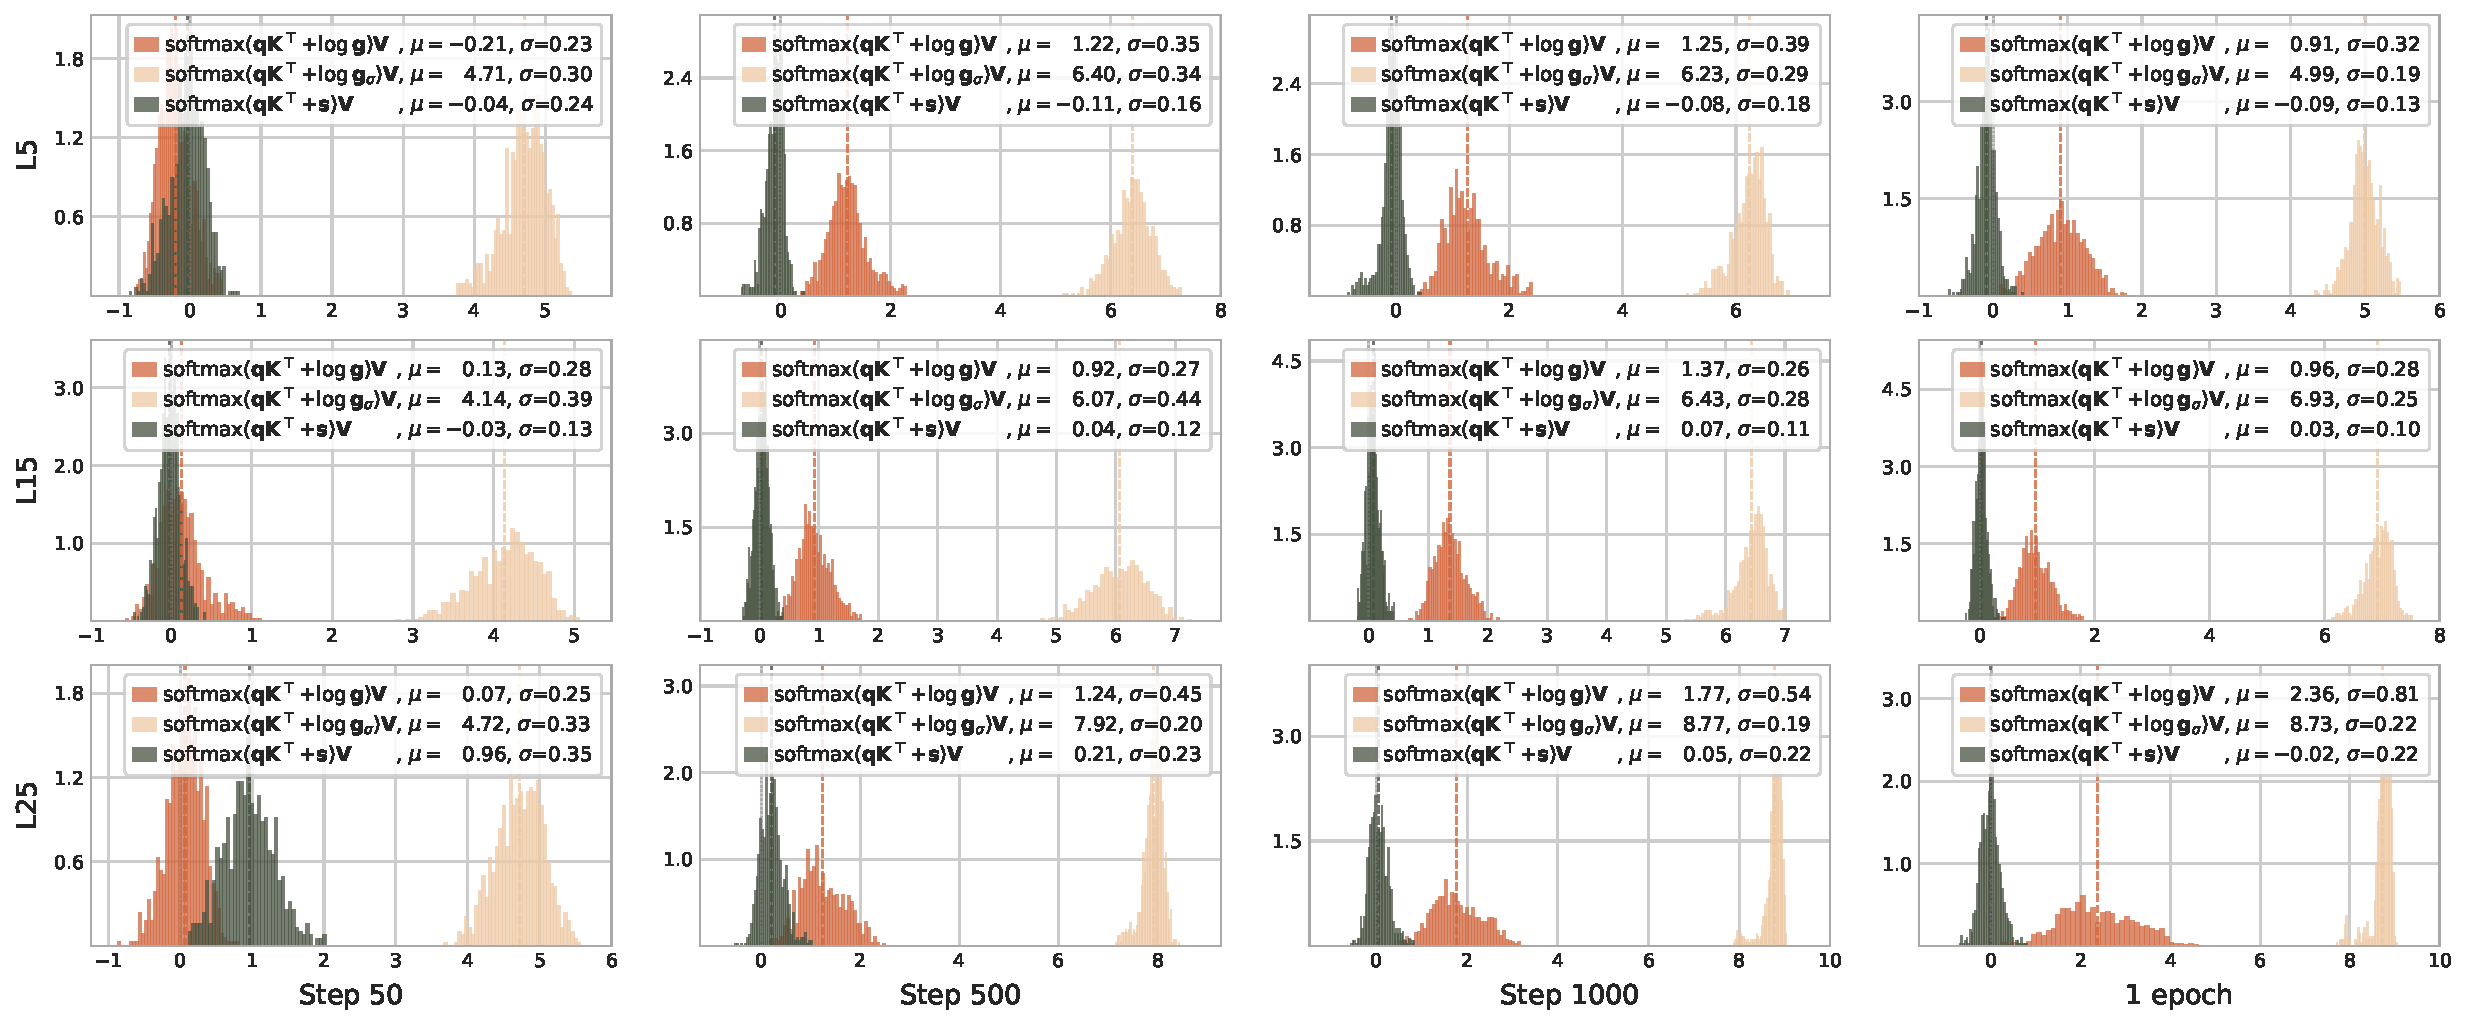
\includegraphics[width=0.99\linewidth]{sec/fig/logits_distribution_L5_L15_L25_overlay1.pdf}
    \caption{
        Evolution of selector logits $\mathbf{s}$ under softmax, sigmoid gating and raw-logit injection in different layers.
        Sigmoid gating saturates historical gates toward one, while raw injection collapses logits toward zero with reduced variance. Thus, both transformations approach effectively ungated attention and fail to provide a discriminative signal for learning block rankings. These observations highlight the importance of the competitive nature of softmax normalization in avoiding such trivial solutions and preserving discriminative block selection.
    }
    \label{fig:logit_dynamic}
\end{figure}

\paragraph{Ranking preservation.}
The key difference is whether the forward pass preserves the continuous ranking or collapses it into a binary Top-$K$ mask.
Let $z_i=\mathbf{q}\mathbf{k}_i^\top$ denote the attention logit of token $i$, where $\mathbf{k}_i$ is its key vector, and let $b(i)$ index the block that token $i$ belongs to.
Soft gating keeps every block under a single normalizer that sums over all tokens, so each attention weight stays bounded.
Hard gating instead relies on STE for a differentiable backward: its forward normalizer sums only over the selected set $\mathcal{S}$, and a dropped block $m\notin\mathcal{I}$ is ranked by the attention mass its tokens would receive under this restricted normalizer, from which its own tokens are absent:
\begin{equation}
    \tilde p_i^{soft}
    =
    \frac{g_{b(i)}\exp(z_i)}{\sum_j g_{b(j)}\exp(z_j)}
    \le 1,
    \qquad
    \tilde p_i^{hard}
    =
    \frac{\exp(z_i)}{\sum_{j\in\mathcal{S}}\exp(z_j)}
    \le
    \exp\!\left(z_i-\max_{j\in\mathcal{S}}z_j\right).
    \label{eq:rank_unbounded}
\end{equation}
The soft weight $\tilde p_i^{soft}$ is always bounded, while the hard weight $\tilde p_i^{hard}$ has no upper bound and grows exponentially once a dropped block outscores the selected set. 
Since the gate gradient satisfies $dg_m\propto p_i$ (Equation~\ref{eq:gate_posi}), these unbounded weights are directly translated into large gradients. 
Early in training, the randomly initialized selector frequently leaves high-score blocks outside Top-$K$, causing the contributions from dropped blocks, tokens, and heads to accumulate and producing gradient norms that are orders of magnitude larger than those of soft gating.


\begin{figure}[!t]
    \centering
    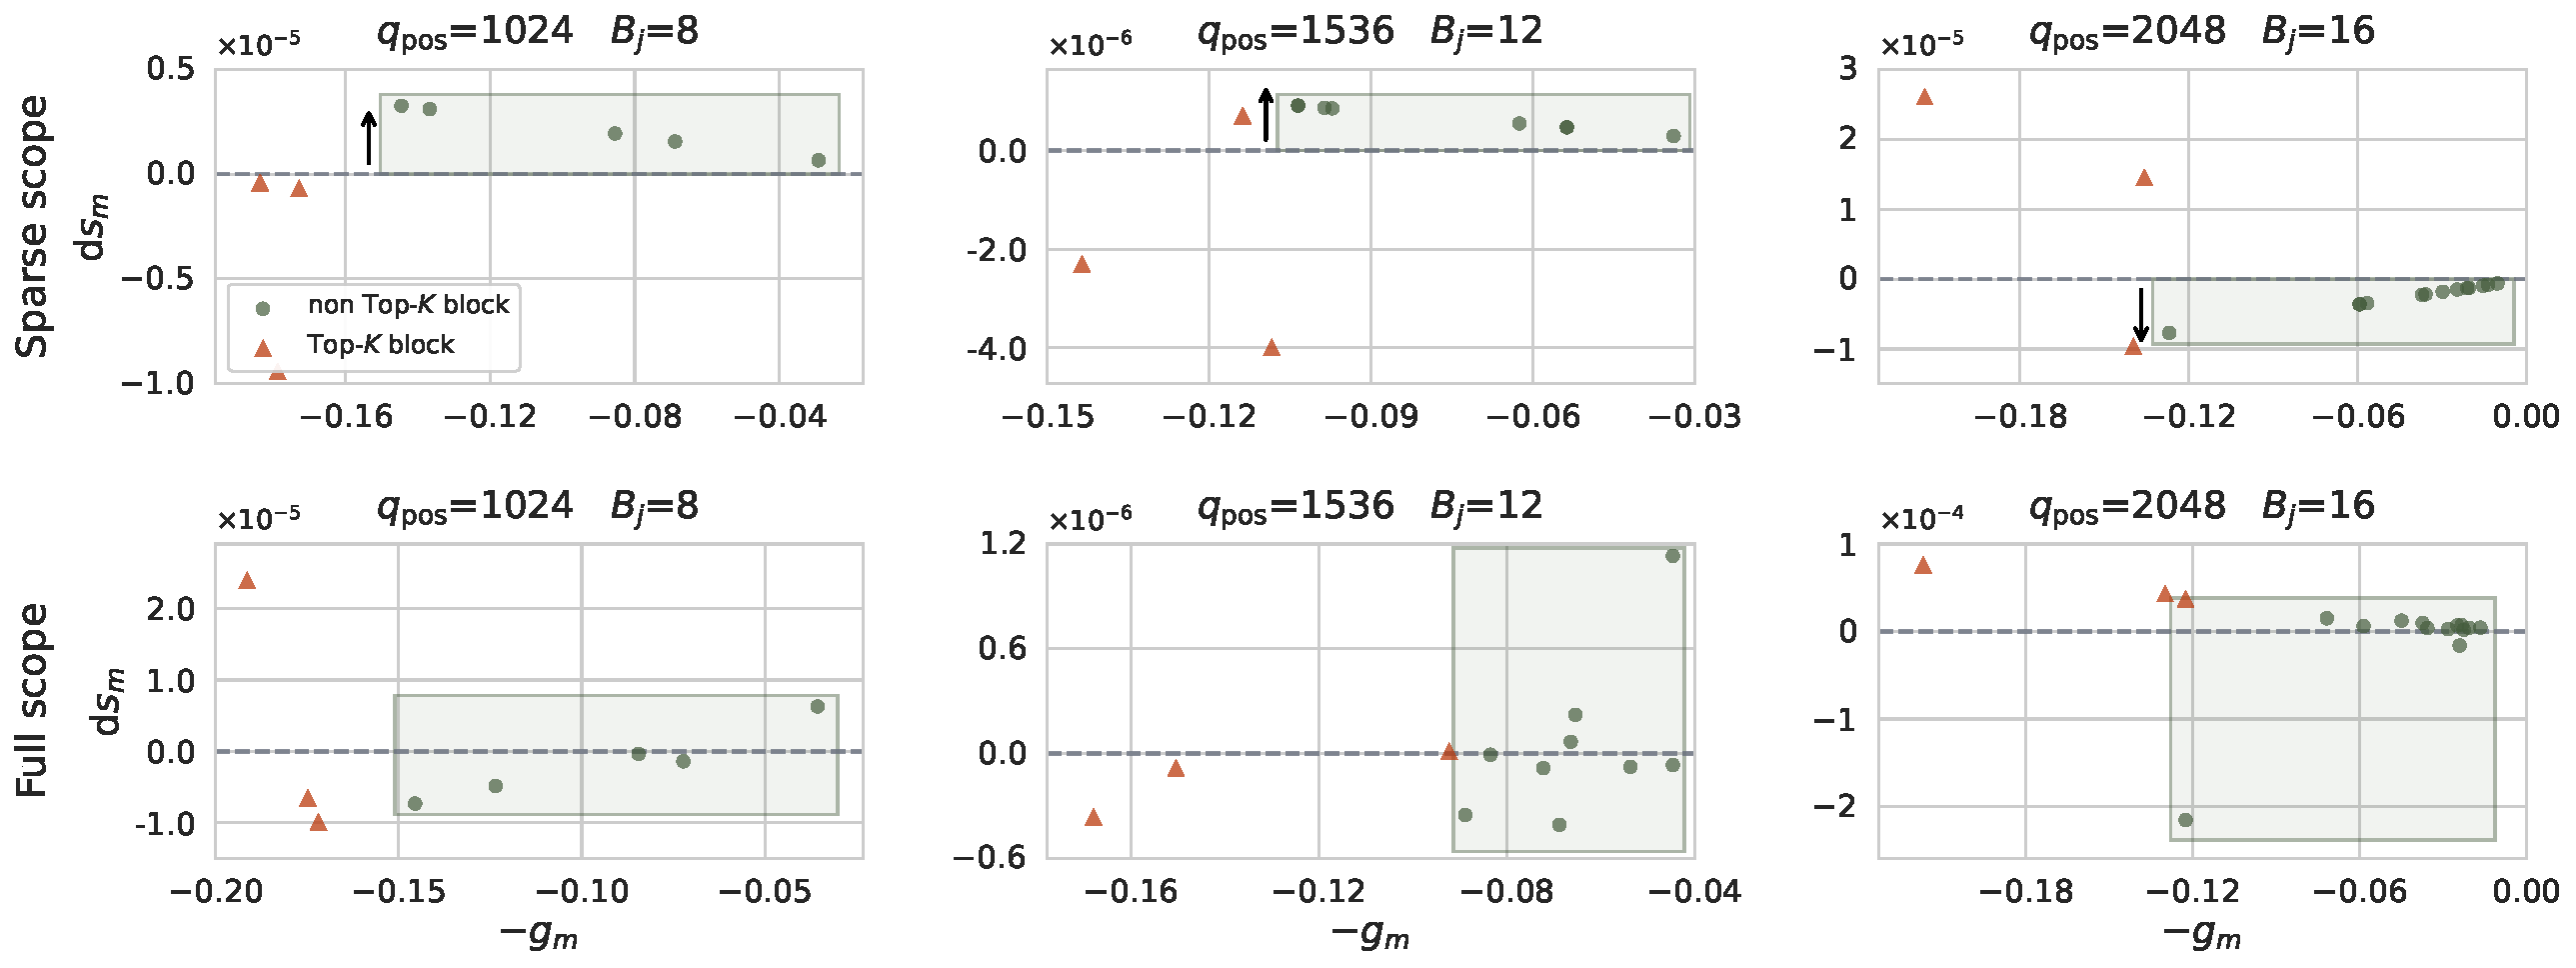
\includegraphics[width=0.98\linewidth]{sec/fig/scatter_dlogits_vs_soft_combined_refined.pdf}
    \caption{Gradient behavior under sparse and full training scopes with Top-$K$ of 3.
For non Top-$K$ blocks, sparse scope training yields noisy and highly correlated gradients, with gradients of these unselected blocks simultaneously being either positive or negative across blocks, ignoring their own importance scores ($x$-axis). This provides a less informative optimization signal and leads to less efficient gate optimization than full scope training.
    }
    \label{fig:ds_vs_softs}
\end{figure}


\paragraph{Training scope.}
The key difference is whether non-Top-$K$ blocks receive \textit{independent gradient signals}.
Under sparse scope, only the current Top-$K$ blocks participate in attention.
A block outside the selected set therefore has no direct gate gradient, even if its score may still change indirectly through the $\operatorname{softmax}$ normalization over selector scores.
This indirect update does not evaluate the content of the unselected block itself. For $\phi(\cdot)=\operatorname{softmax}(\cdot)$, consider an unselected block $B_m$ with $m\notin\mathcal{I}$.
Gradients under sparse and full scope are
\begin{equation}
ds_m^{sparse}
=
-g_m
\cdot
\underbrace{\sum_{\ell\in\mathcal{I}} g_\ell dg_\ell}_{\text{Top-$K$ blocks}},
\qquad
ds_m^{full}
=
-g_m
\cdot
\underbrace{
\bigg(
-dg_m
+
\sum_{\ell=1}^{C} g_\ell dg_\ell
\bigg)}_{\text{own signal + full normalization}}.
\label{eq:scope_grad}
\end{equation}
As shown in \Cref{fig:ds_vs_softs}, sparse scope updates an unselected block only through selected blocks, while full scope gives it its own  gradient $dg_m$, allowing its score to be adjusted based on its own content.

Empirically, as shown by settings (9) and (10) in \Cref{tab:ablation_main}, sparse scope starts worse than full scope but gradually catches up, reaching comparable final performance. This trend holds across model scales and budgets (Appendix~\ref{app:scope_final}).
Given its lower training cost, we therefore rely mainly on sparse scope in our subsequent experiments.
We provide the whole gradient derivations in Appendix 
\ref{app:derivation}.

\subsection{Instantiating Simple Attention Sparsification}
\label{sec:ranksparse}

Based on the above analysis, \our adopts four design choices: \emph{1)} inner $\operatorname{softmax}$ gate injection, \emph{2)} $\operatorname{softmax}$ gate activation, \emph{3)} soft gate to keep ranking information, \emph{4)} sparse scope during training.
Given the query $\mathbf{q}$, the selector computes relevance scores for the historical blocks
$\mathbf{s}
=
\mathcal{R}_{\theta}
\left(
\mathbf{q},
\{\mathbf{K}_{B_m}\}_{m=1}^{C}
\right).$
The scores are converted into normalized gates $\mathbf{g}=\operatorname{softmax}(\mathbf{s})$, and the Top-$K$ historical blocks are selected as $\mathcal{I}=\text{Top-}K(\mathbf{g},K)$. We define the attended token set as $\mathcal{S}=B_0\cup\bigcup_{m\in\mathcal{I}}B_m$, including the always-retained current block $B_0$, and broadcast the selected block gates to the token-level gate $\mathbf{g}_{\mathcal{S}}$ aligned with the attention logits. The resulting attention computation used during training is given by
\begin{equation}
\mathbf{o}_{\our}
=
\operatorname{softmax}
\left(
    \mathbf{q}\mathbf{K}^{\top}_{\mathcal{S}}
    +
    \log\mathbf{g}_{\mathcal{S}}
\right)
\mathbf{V}_{\mathcal{S}}.
\label{eq:ours_train}
\end{equation}
Thus, the selected historical blocks receive normalized log-gate biases, whereas the current block remains unbiased with a unit gate, which instantiates the differentiable continuous gating illustrated in \Cref{fig:motivation}b.
At inference time, the learned ranking is discretized into Top-$K$ block indices.
Algorithms~\ref{alg:ours_train} and~\ref{alg:ours_infer} summarize the training and inference procedures, respectively.

\begin{figure}[!t]
\centering
\newcommand{\algstrut}{\rule[-1.0ex]{0pt}{3.0ex}}
\begin{minipage}[t]{0.48\textwidth}
\begin{algorithm}[H]
\caption{\our Training Step}
\label{alg:ours_train}
\begin{algorithmic}[1]
\Require \algstrut $\mathbf{q},\mathbf{K},\mathbf{V}$, selector $\mathcal{R}_{\theta}$, budget $K$
\State \algstrut $\mathbf{s}=\mathcal{R}_{\theta}\left(\mathbf{q},\{\mathbf{K}_{B_m}\}_{m=1}^{C}\right)$
\State \algstrut $\mathbf{g}=\operatorname{softmax}(\mathbf{s})$
\State \algstrut $\mathcal{I}=\text{Top-}K(\mathbf{g},K)$, $\mathcal{S}=B_0\cup\bigcup_{m\in\mathcal{I}}B_m$
\State \algstrut $\mathbf{o}=\operatorname{softmax}(\mathbf{q}\mathbf{K}^{\top}_{\mathcal{S}}+\log\mathbf{g}_{\mathcal{S}})\mathbf{V}_{\mathcal{S}}$
\State \algstrut Update $\theta$ with $\nabla_{\theta}\mathcal{L}_{\mathrm{LM}}$
\State \algstrut \Return $\mathcal{R}_{\theta}$
\end{algorithmic}
\end{algorithm}
\end{minipage}
\hfill
\begin{minipage}[t]{0.48\textwidth}
\begin{algorithm}[H]
\caption{\our Inference Step}
\label{alg:ours_infer}
\begin{algorithmic}[1]
\Require \algstrut $\mathbf{q},\mathbf{K},\mathbf{V}$, selector $\mathcal{R}_{\theta}$, budget $K$
\State \algstrut $\mathbf{s}=\mathcal{R}_{\theta}\left(\mathbf{q},\{\mathbf{K}_{B_m}\}_{m=1}^{C}\right)$
\State \algstrut $\mathcal{I}=\text{Top-}K(\mathbf{s},K)$
\State \algstrut $\mathcal{S}=B_0\cup\bigcup_{m\in\mathcal{I}}B_m$
\State \algstrut $\mathbf{o}=\operatorname{softmax}\left(\mathbf{q}\mathbf{K}_{\mathcal{S}}^{\top}\right)\mathbf{V}_{\mathcal{S}}$
\State \algstrut Forward to obtain next token logits
\State \algstrut \Return next token
\end{algorithmic}
\end{algorithm}
\end{minipage}
\label{fig:ours_algorithm}
\end{figure}


\paragraph{Kernel Design.}
SAS training computes sparse scope attention, $\operatorname{softmax}(\mathbf{q}\mathbf{K}^\top_{\mathcal{S}}+\log\mathbf{g}_{\mathcal{S}})\mathbf{V}_{\mathcal{S}}$, where $\log\mathbf{g}_{\mathcal{S}}$ contains normalized log-gate biases for selected historical blocks and zero bias for the always-retained current block.
The selected historical set is encoded by a per-query threshold on the gate: a block is active when its log gate reaches the threshold, which realizes the Top-$K$ selection $\mathcal{I}$ without an explicit sort.
FlashAttention \cite{dao2022flashattention} kernels neither support injecting such per-block gates inside the tiled $\operatorname{softmax}$ nor skipping blocks according to a learned gate.
A naive implementation materializes the gated attention matrix, incurring prohibitive memory overhead.


We implement a FlashAttention-style Triton \cite{tillet2019triton} kernel that fuses the block gate into the tile-level $\mathbf{q}\mathbf{K}_{\mathcal{S}}^\top$ computation.
During the streaming scan over key--value tiles, the kernel adds the normalized log gate to the attention logits of each selected historical block, masks out non-selected historical blocks, leaves the always-retained current block unbiased, and performs the standard online $\operatorname{softmax}$ update.
The backward pass accumulates block-level log-gate gradients by summing the attention-logit gradients within each selected historical block.
This kernel keeps the sparse training scope while avoiding attention-matrix materialization and retaining FlashAttention-style memory efficiency. Pseudocode is provided in Appendix~\ref{sec:app_kernel}.
